%===============================================================================
%
%===============================================================================
\section{Les registres}

   La notion de {\em registre} permet de définir dans ManuX des
structures de données pouvant être utilisées pour paramétrer les
différents sous-systèmes.

   L'objectif est de permettre en particulier de faire passer lors du
{\em boot} au noyau des paramètres qui pourront écraser les valeurs par
défaut de certaines variables.

   On pensera par exemple à un masque de débogage ou à une adresse
{\sc ip} définie en dur dans le code mais que l'on pourra changer {\em
  via} la commande de {\em boot}.

   À titre d'exemple, le noyau ManuX utilise une variable qui contient
un masque permettant de définir quels messages sont affichés durant
l'exécution du système.

   Voici l'exécution du système alors que cette variable est
initialisée à sa valeur par défaut ({\tt 0x3}) qui n'active que
l'affichage des messages de démarrage et les éventuels messages
d'erreur~:

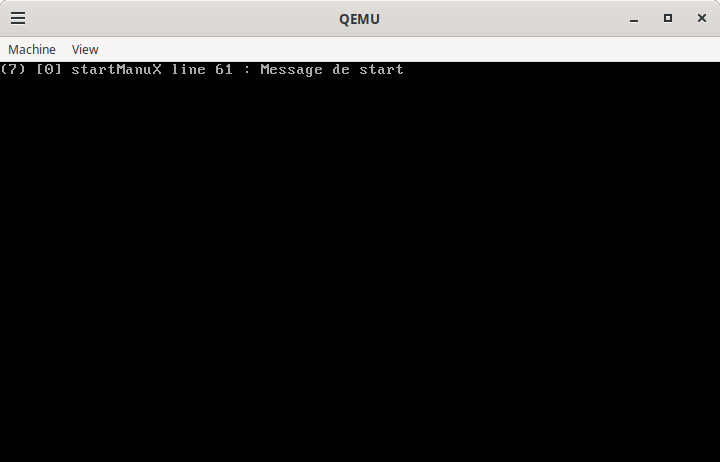
\includegraphics{images/reg-param-1-res.png}

   Voici maintenant le même noyau démarré puis exécuté avec une valeur
différente de sorte à afficher les messages de type ``à faire''. La
première image montre l'utilisation du {\em bootloader} pour modifier
la valeur de la variable~: 

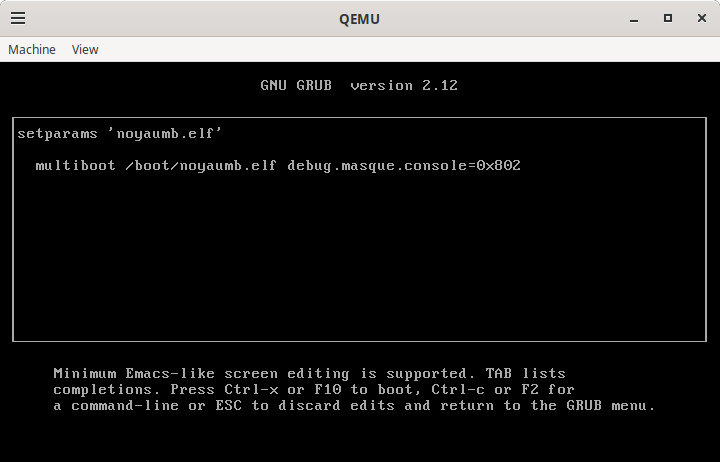
\includegraphics{images/reg-param-802.png}

   Nous avons ici choisi la valeur {\tt 0x802} qui active l'affichage
des message ``à faire'' ({\tt 0x800})et les messages de démarrage
({\tt 0x2}). L'image suivante montre alors l'exécution du noyau~:

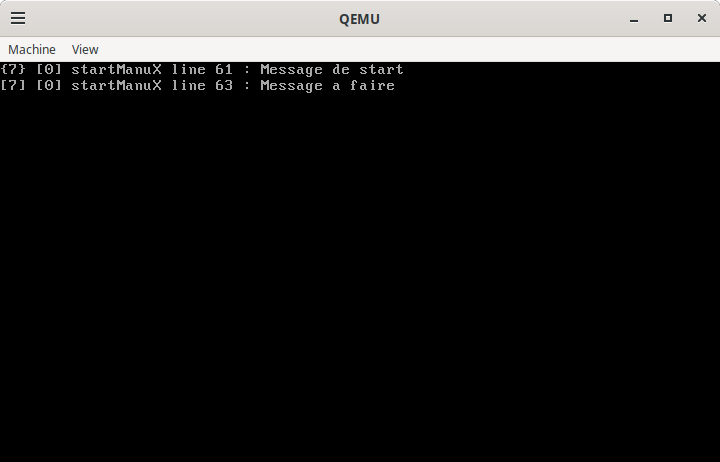
\includegraphics{images/reg-param-802-res.png}

   C'est au travers de l'utilisation d'un registre que cette variable
est manipulée ici.

%-------------------------------------------------------------------------------
% Définition d'un registre
%-------------------------------------------------------------------------------
\subsection{Définition d'un registre}

   Un registre est une abstraction permettant de stocker des
informations dans une structure arborescente. L'objectif est le
paramétrage d'un (sous-)système donc les informations stockées sont
simplement de courtes chaînes de caractères.

   Le principe est que chaque entrée dans le registre (que nous
appellerons un {\em paramètre}) est liée à une variable au travers
d'une fonction de mise-à-jour de la variable.

   La variable ne doit alors {\em jamais être modifiée directement},
mais uniquement au travers d'une modification du paramètre
correspondant dans le registre. La variable sera alors mise-à-jour
automatiquement au travers de la fonction associée.

%-------------------------------------------------------------------------------
% Implantation
%-------------------------------------------------------------------------------
\subsection{Implantation d'un registre}

   Les registres sont définis dans \fichier{manux}{registre}{h} et
implantés dans \fichier{lib}{registre}{c}.

La fonction principale pour peupler le registre est la suivante

\begin{lstlisting}
void registreAffecterParametre(registre * reg,
                               char * valeur,
                               void * prive,
                               registreMiseAJour miseAJour,
                               ...);
\end{lstlisting}
   
%-------------------------------------------------------------------------------
%
%-------------------------------------------------------------------------------
\subsection{Le registre système}

   Le registre {\tt ManuX-Param} est destiné à contenir les paramètres
du noyau ManuX.

%-------------------------------------------------------------------------------
%
%-------------------------------------------------------------------------------
\subsection{Exemple d'utilisation}

   Un exemple d'utilisation simple du registre est donné dans
\fichier{multiconf}{registre}{h}. Le code est dans le fichier
\fichier{noyau}{main-registre}{c}.

   Dans ce fichier, 4 paramètres sont initialisés de différentes
façons :

\begin{itemize}
   \item{\tt a} reçoit une valeur au démarage, puis sa fonction de
     mise-à-jour lui est affectée avec une valeur par défaut, qui
     n'est donc pas utilisée.
   \item{\tt b} reçoit une valeur au démarage, puis sa fonction de
     mise-à-jour lui est affectée sans valeur par défaut.
   \item{\tt c} ne reçoit pas de valeur au démarage, puis sa fonction
     de mise-à-jour lui est affectée avec une valeur par défaut, qui
     est donc utilisée.
   \item{\tt d} reçoit une valeur au démarage, puis sa fonction de
     mise-à-jour lui est affectée avec une valeur par défaut, qui
     n'est donc pas utilisée, mais une nouvelle valeur lui est ensuite
     affectée, qui est celle finalement utilisée.     
\end{itemize}

   Par soucis de simplicité, on n'utilise pas ici les outils de {\em boot}
pour passer des paramètres, mais cela ne change rien.
